\section{Forward-JWKB Approximation\label{sec2}}
%%%%%%%%%%%%%%%%%%%%%%%%%%%%%%%%%%%%%%%%%%%%%%%%%%%%%%%%%%%%%%%%%%%%%%%%%%%%%%%
In order to be concrete, we consider a four-point scattering event with two non-identical, massive, scalar particles that exchange massless, scalar quanta via a cubic interaction. The $s$-channel process is elastic:
\begin{equation}
	\Phi_{1}(p_{1}) + \Phi_{2}(p_{2}) \longrightarrow \Phi_{1}(p_{3}) + \Phi_{2}(p_{4}).
	\label{ScaProc}
\end{equation}
In this channel, the center-of-momentum energy is given by $\sqrt{s}$ and the magnitude of the momentum transfer is $\sqrt{-t}$. More details about kinematics can be found in Appendix \ref{app1}.
%%%%%%%%%%%%%%%%%%%%%%%%%%%%%%%%%%%%%%%%%%%%%%%%%%%%%%%%%%%%%%%%%%%%%%%%%%%%%%%
\subsection{Regge Limit}
%%%%%%%%%%%%%%%%%%%%%%%%%%%%%%%%%%%%%%%%%%%%%%%%%%%%%%%%%%%%%%%%%%%%%%%%%%%%%%%
Consider the one-loop contribution from the box diagram:
\begin{equation}
	\vcenter{\hbox{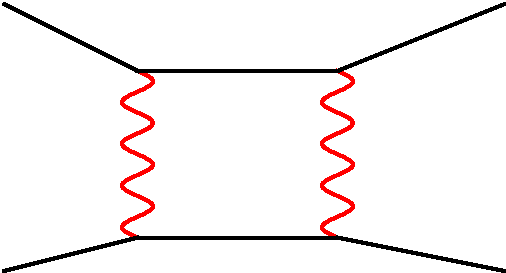
\includegraphics[scale=0.4]{figures/box.pdf}\put(-110,50){$1$} \put(-110,-2){$2$} \put(3,50){$3$} \put(5,-4){$4$}}} \label{BoxDiagram}
\end{equation}
The scattering amplitude from this contribution can be written as an integral over Feynman variables:
\begin{equation}
	\mathcal{A}_{\text{box}}(s, t) \sim g^{4} \Gamma\left( \frac{8 - D}{2} \right) \int\limits_{0}^{1} \int\limits_{0}^{1} \int\limits_{0}^{1} \int\limits_{0}^{1} \mathrm{d}f_{31} \mathrm{d}f_{42} \mathrm{d}f_{12} \mathrm{d}f_{34} \, \frac{\delta(1 - f_{12} - f_{34} - f_{31} - f_{42})}{[B(s, t|f_{ij})]^{(8 - D)/2}};
	\label{BoxIntegral}
\end{equation}
where
\begin{equation}
	B(s, t|f_{ij}) \equiv m_{1}^{2} f_{31}^{2} + m_{2}^{2} f_{42}^{2} + (m_{1}^{2} + m_{2}^{2} - s) f_{31} f_{42} - t f_{12} f_{34}.
\end{equation}
This expression is valid for generic values of $s$ and $t$. However, in the Regge limit
\begin{equation}
	\frac{t}{m_{1} m_{2}} \rightarrow \infty, \qquad \frac{s}{m_{1} m_{2}} \text{ fixed,} \qquad \frac{m_{1}}{m_{2}} \text{ fixed,}
	\label{ReggeLimit}
\end{equation}
the integrals in (\ref{BoxIntegral}) can be evaluated with asymptotic methods \cite{SMatrixBook}. In $D = 4$ one finds
\begin{equation}
	\mathcal{A}_{\text{box}}(s, t) \sim \frac{g^{2}}{t} \left[ g^{2} \rho(s) \right] \log{\left( -\frac{t}{2\mu^{2}} \right)};
\end{equation}
where
\begin{equation}
	\rho(s) \equiv \int\limits_{0}^{1} \frac{\mathrm{d}f}{m_{2}^{2} + (m_{1}^{2} - m_{2}^{2} - s)f + s f^{2}} = \frac{1}{\sqrt{-\Lambda_{12}}} \log{\left[ \frac{m_{1}^{2} + m_{2}^{2} - s - \sqrt{\Lambda_{12}}}{m_{1}^{2} + m_{2}^{2} - s + \sqrt{\Lambda_{12}}} \right]}.
	\label{LeeSawyer}
\end{equation}
with $\Lambda_{12}$ the K\"{a}ll\'{e}n function,
\begin{equation}
	\Lambda_{12} \equiv [s - (m_{1} - m_{2})^{2}][s - (m_{1} + m_{2})^{2}].
\end{equation}
Actually, this result for the one-loop scalar box in the Regge limit agrees with the exact result \cite{PvN,tHVelt}. The logarithm term in (\ref{LeeSawyer}) can be recognized as twice the sum of the rapidities of the incoming states in the center-of-momentum frame (see Appendix \ref{app1}).

Diagrammatically, the Regge limit turns the square polygon in (\ref{BoxDiagram}) into a digon made of matter lines, multiplied by a certain prefactor:
\begin{equation}
	\vcenter{\hbox{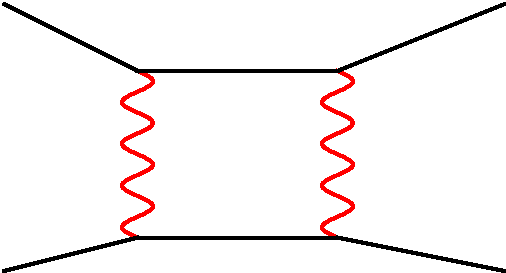
\includegraphics[scale=0.4]{figures/box.pdf}}} \quad \longrightarrow \quad (\cdots)\vcenter{\hbox{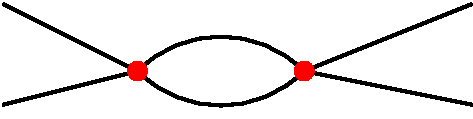
\includegraphics[scale=0.4]{figures/regge_box.pdf}}}
	\label{ReggeBox}
\end{equation}
Whereas the external lines remain unchanged, the internal lines on the left-hand side are matter propagators in $D$ dimensions, while those on the right-hand side are matter propagators in $D-2$ dimensions. Similarly, the double box diagram becomes the concatenation of two matter digons:
\begin{equation}
	\vcenter{\hbox{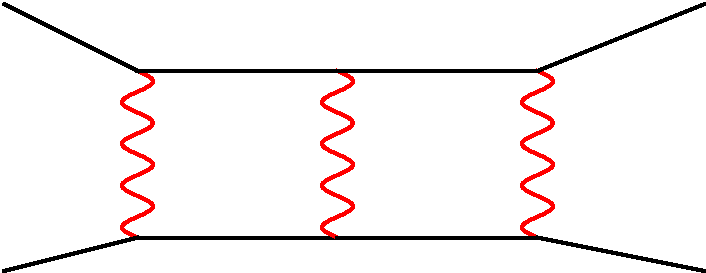
\includegraphics[scale=0.4]{figures/doublebox.pdf}}} \quad \longrightarrow \quad (\cdots)\vcenter{\hbox{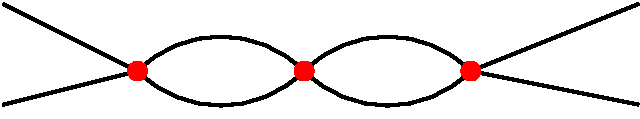
\includegraphics[scale=0.4]{figures/regge_doublebox.pdf}}} \label{ReggeDoubleBox}
\end{equation}
In this way the sum over ladder diagrams becomes much simpler in the Regge limit \cite{LeeSawyer}:
\begin{equation}
	\mathcal{A}_{\text{ladders}}(s, t) \sim g^{2} \Gamma[-R(s)] \left(- \frac{t}{2 \mu^{2}} \right)^{R(s)}, \qquad R(s) = -1 + g^{2} \rho(s) \label{ladders}.
\end{equation}
Note that the Regge limit takes us outside of the physical scattering region of the $s$-channel process. One way to motivate the use of the Regge limit is to consider the (inelastic) $t$-channel process:
\begin{equation}
	\Phi_{1}(p_{1}) + \bar{\Phi}_{1}(\bar{p}_{2}) \longrightarrow \bar{\Phi}_{2}(\bar{p}_{3}) + \Phi_{2}(p_{4}).
\end{equation}
In this channel, the center-of-momentum energy is $\sqrt{t}$ and the magnitude of the momentum transfer is $\sqrt{-s}$ (after crossing from the $s$-channel). Thus, the Regge limit (\ref{ReggeLimit}) in the $s$-channel corresponds to the high-energy and fixed-momentum transfer regime in the $t$-channel. Note that this regime involves light masses, or via $\lambda_{j} = \hbar / m_{j}$, large Compton wavelengths. That is, the Regge limit involves distances that are much smaller than the Compton wavelengths (microscopic regime). This is the same regime as taking $\hbar \rightarrow \infty$, so in a way the Regge limit takes us deep into the quantum realm. Indeed, the spectrum of bound states that follows from the poles of the Euler Gamma function in (\ref{ladders}) involves the exact one-loop (quantum) result (\ref{LeeSawyer}), and diagrams like (\ref{ReggeDoubleBox}) involve vertices with only internal (quantum) lines attached to them.

Systems where the interaction is mediated by massive quanta can be considered in a similar way, since the Regge limit renders the massive mediator effectively massless, and thus the result is the same. That is, the Regge limit is insensitive to the mediator's mass.
%%%%%%%%%%%%%%%%%%%%%%%%%%%%%%%%%%%%%%%%%%%%%%%%%%%%%%%%%%%%%%%%%%%%%%%%%%%%%%%
\subsection{Forward-JWKB Regime}
%%%%%%%%%%%%%%%%%%%%%%%%%%%%%%%%%%%%%%%%%%%%%%%%%%%%%%%%%%%%%%%%%%%%%%%%%%%%%%%
In contrast to the Regge limit (\ref{ReggeLimit}), we \textit{define} the forward-JWKB limit by
\begin{equation}
	{-\frac{t}{m_{1} m_{2}}} \rightarrow 0^{+}, \qquad \frac{s}{m_{1} m_{2}} \text{ fixed,} \qquad \frac{m_{1}}{m_{2}} \text{ fixed.} \label{fJWKBLimit}
\end{equation}
This regime is the same as restricting to small (but physical) scattering angles. Note that the Regge limit corresponds to unphysical scattering angles (i.e. $z_{s} \rightarrow \infty$). From (\ref{fJWKBLimit}) it follows that $-t/s \rightarrow 0^{+}$, meaning that the center-of-momentum energy $\sqrt{s}$ is much larger than the magnitude of the momentum transfer $\sqrt{-t}$. In other words, this is a high-energy approximation (in the $s$-channel, the Regge limit is a low-energy approximation because $t/s \rightarrow \infty$). Moreover, it also follows that $-t/m_{1}^{2} \rightarrow 0^{+}$ and $-t/m_{2}^{2} \rightarrow 0^{+}$, which mean that the external masses $m_{j}$ are very large compared to $\sqrt{-t}$. Thus, this regime involves heavy masses, or via $\lambda_{j} = \hbar / m_{j}$, short Compton wavelengths. Hence, the forward-JWKB limit involves distances that are much larger than the Compton wavelengths (macroscopic regime), which coincides with the limit $\hbar \rightarrow 0$: the (semiclassical) JWKB limit.

Although we are not going to use perturbative second-quantized Feynman diagrams, it is somewhat illuminating to see what happens to the ladder series in the forward-JWKB limit. In contrast to (\ref{ReggeBox}), the one-loop box becomes a digon made with mediator lines,
\begin{equation}
	\vcenter{\hbox{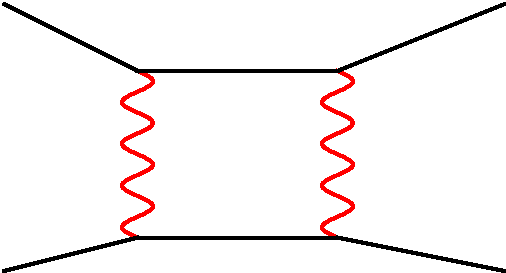
\includegraphics[scale=0.4]{figures/box.pdf}}} \quad \longrightarrow \quad (\cdots)\vcenter{\hbox{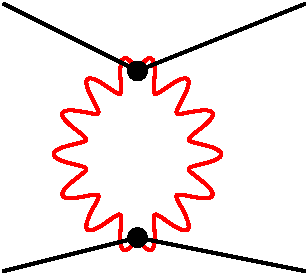
\includegraphics[scale=0.4]{figures/fjwkb_box.pdf}}} \label{fJWKBBox}
\end{equation}
and similarly for the two-loop double box:
\begin{equation}
	\vcenter{\hbox{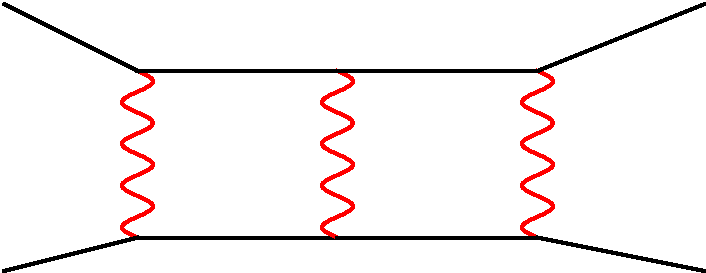
\includegraphics[scale=0.4]{figures/doublebox.pdf}}} \quad \longrightarrow \quad (\cdots)\vcenter{\hbox{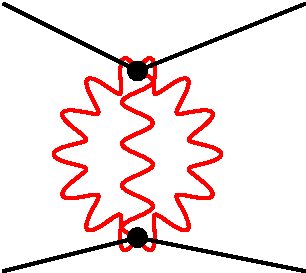
\includegraphics[scale=0.4]{figures/fjwkb_doublebox.pdf}}} \label{fJWKBDoubleBox}
\end{equation}
We see that the structure of the forward-JWKB ladders is very different from the Regge ladders. Indeed, the forward-JWKB ladders do not involve any internal vertices and only involve internal mediator lines (which, like the internal matter lines in the Regge ladders, live in $D - 2$ dimensions). At face value, the forward-JWKB approximation does not make the evaluation of the integrals in (\ref{BoxIntegral}) any easier. This is why we do not explicitly prove (\ref{fJWKBBox}) and (\ref{fJWKBDoubleBox}) for generic theories. However, in \S\ref{sec6} we obtain a scattering amplitude in $D = 3$ using the forward-JWKB approximation that agrees with the expectations from (\ref{fJWKBBox}), (\ref{fJWKBDoubleBox}) and beyond.